\documentclass{article}

\usepackage{fancyhdr}
\usepackage{extramarks}
\usepackage{amsmath}
\usepackage{amsthm}
\usepackage{amsfonts}
\usepackage{tikz}
\usepackage{graphicx} %插入图片的宏包
\usepackage{float} %设置图片浮动位置的宏包
% \usepackage{pythonhighlight}
% \usepackage{subfigure} %插入多图时用子图显示的宏包
% \usepackage[plain]{algorithm}
% \usepackage{algpseudocode}

% \usetikzlibrary{automata,positioning}

%
% Basic Document Settings
%

\topmargin=-0.45in
\evensidemargin=0in
\oddsidemargin=0in
\textwidth=6.5in
\textheight=9.0in
\headsep=0.25in

\linespread{1.1}

\pagestyle{fancy}
\lhead{\hmwkAuthorName}
\chead{\hmwkClass\ : \hmwkTitle}
\rhead{\firstxmark}
\lfoot{\lastxmark}
\cfoot{\thepage}

\renewcommand\headrulewidth{0.4pt}
\renewcommand\footrulewidth{0.4pt}

\setlength\parindent{0pt}


%代码格式设置



%
% Create Problem Sections
%

\newcommand{\enterProblemHeader}[1]{
    \nobreak\extramarks{}{Problem \arabic{#1} continued on next page\ldots}\nobreak{}
    \nobreak\extramarks{Problem \arabic{#1} (continued)}{Problem \arabic{#1} continued on next page\ldots}\nobreak{}
}

\newcommand{\exitProblemHeader}[1]{
    \nobreak\extramarks{Problem \arabic{#1} (continued)}{Problem \arabic{#1} continued on next page\ldots}\nobreak{}
    \stepcounter{#1}
    \nobreak\extramarks{Problem \arabic{#1}}{}\nobreak{}
}

\setcounter{secnumdepth}{0}
\newcounter{partCounter}
\newcounter{homeworkProblemCounter}
\setcounter{homeworkProblemCounter}{1}
\nobreak\extramarks{Problem \arabic{homeworkProblemCounter}}{}\nobreak{}

%
% Homework Problem Environment
%
% This environment takes an optional argument. When given, it will adjust the
% problem counter. This is useful for when the problems given for your
% assignment aren't sequential. See the last 3 problems of this template for an
% example.
%
\newenvironment{homeworkProblem}[1][-1]{
    \ifnum#1>0
        \setcounter{homeworkProblemCounter}{#1}
    \fi
    \section{Problem \arabic{homeworkProblemCounter}}
    \setcounter{partCounter}{1}
    \enterProblemHeader{homeworkProblemCounter}
}{
    \exitProblemHeader{homeworkProblemCounter}
}

%
% Homework Details
%   - Title
%   - Due date
%   - Class
%   - Section/Time
%   - Instructor
%   - Author
%

\newcommand{\hmwkTitle}{Essay Course}
\newcommand{\hmwkDueDate}{Jan 15, 2019}
\newcommand{\hmwkClass}{Functional Programming}
\newcommand{\hmwkClassTime}{Section A}
% \newcommand{\hmwkClassInstructor}{Professor Isaac Newton}
\newcommand{\hmwkAuthorName}{\textbf{RUOPENG XU} }
\newcommand{\hmwkAuthorNum}{\textbf{18M38179} }

%
% Title Page
%

\title{
    \vspace{2in}
    \textmd{\textbf{\hmwkClass:\ \hmwkTitle}}\\
    \normalsize\vspace{0.1in}\small{Due\ on\ \hmwkDueDate\ }\\
    % \vspace{0.1in}\large{\textit{\hmwkClassInstructor\ \hmwkClassTime}}
    \vspace{3in}
}

\author{\hmwkAuthorName\\ \hmwkAuthorNum}
\date{}

\renewcommand{\part}[1]{\textbf{\large Part \Alph{partCounter}}\stepcounter{partCounter}\\}

%
% Various Helper Commands
%

% Useful for algorithms
\newcommand{\alg}[1]{\textsc{\bfseries \footnotesize #1}}

% For derivatives
\newcommand{\deriv}[1]{\frac{\mathrm{d}}{\mathrm{d}x} (#1)}

% For partial derivatives
\newcommand{\pderiv}[2]{\frac{\partial}{\partial #1} (#2)}

% Integral dx
\newcommand{\dx}{\mathrm{d}x}

% Alias for the Solution section header
\newcommand{\solution}{\textbf{\large Solution}}

% Probability commands: Expectation, Variance, Covariance, Bias
\newcommand{\E}{\mathrm{E}}
\newcommand{\Var}{\mathrm{Var}}
\newcommand{\Cov}{\mathrm{Cov}}
\newcommand{\Bias}{\mathrm{Bias}}

\begin{document}

\maketitle

\pagebreak

\begin{homeworkProblem}
    % questions
Answer either question. If you answer both questions the better answer will be chosen for your evaluation.
\\
\\
1. What’s $\alpha$ -conversion for? 
What kind of problems we will see if $\alpha$ -conversion were not applied? 
Find Min-Caml programs that give incorrect answers in absence of proper $\alpha$-conversion.
\\
\\
Note: You may want to consider the reason why inline.ml refers to Alpha.g.
\\
\\
\\
2. Are optimization modules interdependent? Yes, but in what way? Find a pair of optimization modules 
A and B such that for a program P, B is effective when it is applied after A:
\\
\\
$\exists  P.B(P) = P$ but $B(A(P))\neq A(P) $

% 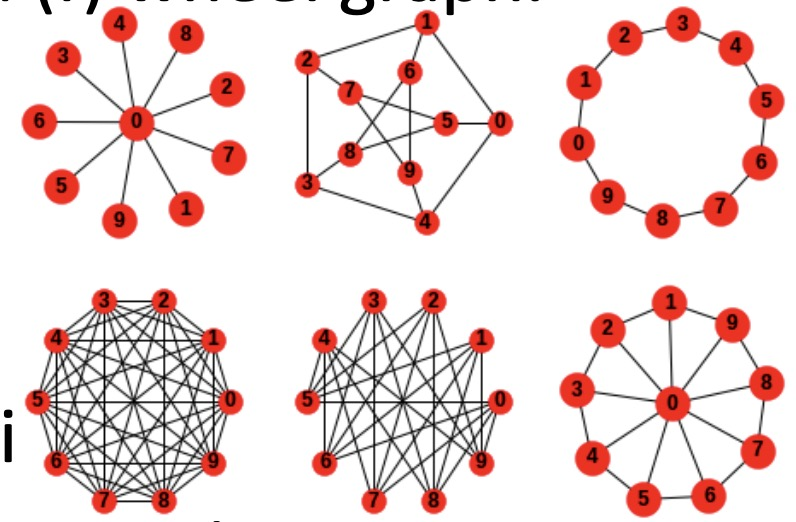
\includegraphics[scale=0.3]{quiz6_1.jpg}

\subsection*{Answer for question 1}
\textbf{What’s $\alpha$ -conversion for? }
\\
\\
$\alpha$ -conversion is to assign different names to different variables. If the variables have same names, the process will be complicated.
\\
\\
In  \textit{alpha.ml} : \textit{let find x env = try M.find x env with Not\_found -$>$ x} will find the current binding of x in env, if the binding not exists, it will return x. 
Therefore, in $\alpha$ -conversion, if the binding is already existed, it will find the binding of variables in env and return it, which means this variables need a new name. On the other hand, if can't find the binding, it will return the variable itself, which means it doesn't need a new name. In this way, we can make sure different variables have different names. 
\\
If it find an expression, it will call the \textit{g env} again to assign different names for the variables in the expression.
\\
\\
For example, \textit{let x = 123 in let x = 456 in x + x} will be translated to \textit{let x1 = 123 in let x2 = 456 in x2 + x2}. In first let process, x will be bind to 123 firstly and 456 secondly, there are different bindings so they need have different names. \textit{Id.genid} will count how many times x appears and call g env again and again in next expression. Finally we will get x1 and x2.
\\
\\
\textbf{What kind of problems we will see if $\alpha$ -conversion were not applied? }
\\
\\
If we didn't use $\alpha$ -conversion in inline expansion, this process may be camplicated and the names of variables will be confused. 
\\
\\
Because in the process of inline expansion, min-caml replaces calls to small functions with their bodies. If the size of the cuntion is lesss than a threshold, min-caml replaces formal arguments with actual arguments, and need to copy the function body. Therefore, the variables may be duplicated and must be $\alpha$ -conversion again to make sure they are different.


\end{homeworkProblem}
\pagebreak


\begin{homeworkProblem}
Answer either question. If you answer both questions the better answer will be chosen for your evaluation.
\\
\\
1.Explain in detail the mechanism described in Figure 16, mincaml/overview.pdf.
\\
- Compare this algorithm with two previous algorithms (Figure 14 and Figure 15). Present a Min-Caml code fragment examples that exhibits superiority of the last algorithm.
\\
- For the examples you gave above, estimate the number of make\_closure, apply\_direct, and apply\_closure executed at runtime when the generated code is executed.
\\
\\
2.Explain how min-caml compiler is organized to achieve the goal of being a multi-targeted native code compiler. (A multi-targeted native code compiler can generate native code targeted for different CPU architectures.)



\subsection*{Answer for qustion 1}
In figure.14, function takes the value of its free variable x as an argument, and then the function is returned as a value, and its body is paired with the free variable. When the function is called, its body and the value of the FV are extracted from the closure. This approach generate a closure for every function and it's inefficient.
\\
\\
In figure.15, it separate the function which need closure from those can be called more conventional. It has a set of known functions that can be called dirctly, because they are known do not have free variables. If the function is closure-based, it calls \textit{apply\_closure}, otherwise it calls \textit{apply\_direct}. In this way it distinguish the type of labels from the type of normal variables.
\\
\\
In figure.16, for example, if the defination is \textit{let rec x y1, y2, ... yn = e1 in e2}.Min-caml firstly assume the function has no free variable, and it can be added to known, and the funtion body e1 is converted. After that, if x doesn't have any free variables, it convert e2. If x has free variables, min-caml rewind the value of know and the reference of top function. Finally, if x never appears as a variable in e2, min-caml omit the closure creation for x.
\\
\\
For example, if the code is like this:
\\
\\
let rec make\_adder x =\\
let rec adder y = x + y in\\
make\_adder
\\
\\
In the first algorithm, all of the variables will be closure:

\textit{let rec adder y = x + y } becomes (adder,x) as a value V1. Then \textit{let rec make\_adder x = V1} is closured to (make\_adder, ). It does a closure to make\_adder which doesn't has any free variable, so it's inefficient.
\\
\\
What's more, in the second algorithm, 
it knows there are no free variables in make\_adder. 
But make\_adder still need a repreastation as a closure because a user who receives make\_adder does not know in general if it has a free variable or not.
\\
\\
Therefore, in the optimized algorithm, \textit{let rec adder y = x + y } becomes (adder,x) as a value V1 firstly as above. \textit{let rec make\_adder x = V1} is thought to be (make\_adder, ) as V2 temporarily. Beecause there are not any free variables in V2, min-caml omits the creation of the closure, which means we save the time of closure creation. Moreover, it is also represented as a closure, which will not confuse the users.
\\
\\
In this example, the \textit{make\_closure} is called twice for adder and make\_adder, \textit{apply\_closure} is called once for adder, and \textit{apply\_direct} is called once for make\_adder.




\end{homeworkProblem}
\pagebreak





\end{document}
%
% Non sequential homework problems
%

% Jump to problem 18
